
\lecture{Escalonamento de processos}{sched}
\title{\insertlecture}

\frame{\maketitle}

\section{\insertlecture}

%%% CONCEITOS
\def\thetitle{Conceitos básicos}
\title{\thetitle}
\frame{\date{}\author{}\titlepage}

\subsection{\thetitle}

\begin{frame}{Políticas}
  \framesubtitle{Processos limitados por E/S x processador}
\small
  \begin{itemize}
  \item E/S -- processos limitados por E/S gastam a maior parte do
    tempo submetendo ou esperando requisições de E/S. Exemplo:
    Interface Gráfica (interação com mouse, teclado, disco).
  \item Processador -- processos limitados por processador gastam a
    maior parte do seu tempo executando código. Exemplo: geradores de
    chave para criptografia, {\sc Matlab}.
  \end{itemize}
  Esta classificação não é mutuamente exclusiva, pois um processo pode
  exibir ambos comportamentos, como o servidor {\sc X Window} por exemplo.
\bigskip

  \alert{A política de escalonamento em um SO deve satisfazer dois objetivos
  conflitantes: tempo de resposta rápido ao processo (baixa latência)
  e máxima utilização do SO (alta vazão).}

\end{frame}

\begin{frame}{Sequência de atividade processador x E/S}
\begin{center}
  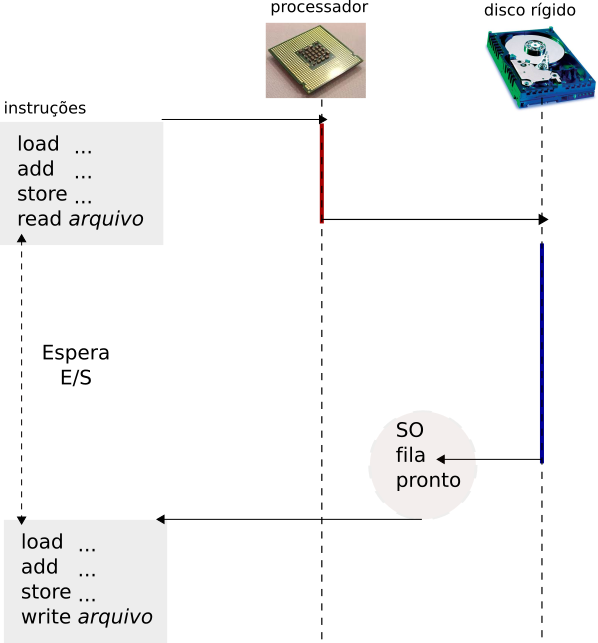
\includegraphics[scale=0.4]{burst-cpu.png}
\end{center}
\end{frame}

\begin{frame}{Escalonamento preemptivo}

  Condições para a tomada de decisão de escalonamento de um processo:

  \begin{enumerate}
  \item<1-| alert@2> \label{sched:es} Processo passa do estado \alert{executando}
    para o estado \alert{esperando}. Por exemplo, como resultado de
    uma requisição de E/S, ou uma chamada de espera pelo término de um
    dos processos filho.
    \item \label{sched:irq}Quando um processo passa do
    estado \alert<1>{executando} para o estado \alert<1>{pronto}. Por
    exemplo, quando ocorre uma interrupção.
     \item \label{sched:endes} Quando um processo passa
    do estado \alert<1>{esperando} para o estado \alert<1>{pronto}. Por
    exemplo, no término da E/S.
    \item<1-| alert@2> \label{sched:end} Quando o processo \alert<1>{termina}.
  \end{enumerate}

\onslide<2>
{\small Para as situações~\ref{sched:es} e \ref{sched:end} não há
  escolha em termos de escalonamento. Este esquema de escalonamento é
  chamada de \alert{não-preemptivo} ou \alert{cooperativo}, foi usado
  no Windows 3.x e Mac OS anterior ao X.}

\end{frame}

\begin{frame}{Despachante}{\em Dispatcher}

{ \color<2>{gray}
Despachante -- componente envolvido no escalonamento do processador
realizando as seguintes funções:
\begin{enumerate}
\color<2>{gray} \item Troca de contexto;
\color<2>{gray}\item Troca para o modo usuário;
\color<2>{gray}\item Desvio para o local apropriado no programa do usuário para
  reiniciar o processo.
\end{enumerate}
}

\onslide<2>
O despachante utiliza um ou vários \alert{políticas de escalonamento}
que normalmente buscam:

\begin{enumerate}
\item Otimizar a utilização do processador;
\item Aumentar a vazão ({\em throughput});
\item Reduzir o tempo de espera (não leva em conta tempo de espera
  devido a requisição de E/S).
\end{enumerate}

  
\end{frame}

%%% ALGORITMOS
\def\thetitle{Algoritmos de escalonamento}
\title{\thetitle}
\frame{\date{}\author{}\titlepage}

\subsection{\thetitle}

\subsubsection{Sistemas em lote}
\label{subsection:batch}

\def\colorone{green!40!black}
\def\colortwo{red!50!black}
\def\colorthree{blue}

\begin{frame}
\frametitle{Primeiro a chegar, primeiro a ser servido (FIFO)}
\framesubtitle{\em FIFO -- first in first out}

\begin{center}
\begin{tabular}{c|c} \hline
  processo & tempo de surto (ms) \\ \hline
  {\color{\colorone} $p_1$} & \only<1>{24} \only<2>{3}\\
  {\color{\colortwo}$p_2$} & 3 \\
  {\color{\colorthree}$p_3$} & \only<1>{3} \only<2>{24} \\ \hline
\end{tabular}
\end{center}

\only<1>{
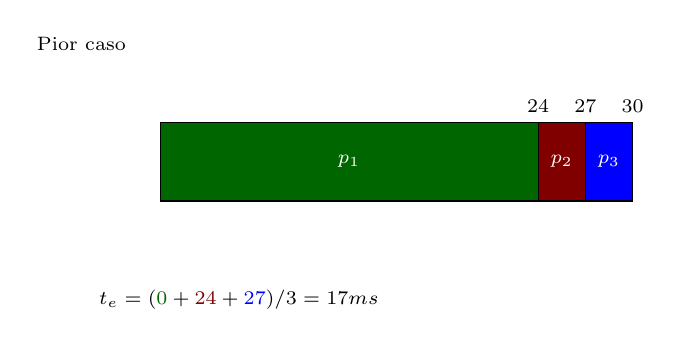
\begin{tikzpicture}[p1/.style={fill=\colorone},
  p23/.style={fill=\colortwo},
  labelsty/.style={midway,text=white}]
  \node at (-1,2) {\alert{Pior} caso};
  \draw[p1] (0,0) rectangle (4.8,1) node[labelsty]{$p_1$} node[above]{24};
  \draw[p23] (4.8,0) rectangle (5.4,1) node[labelsty]{$p_2$} node[above]{27};
  \draw[p23,fill=\colorthree] (5.4,0) rectangle (6,1) node[labelsty]{$p_3$}node[above]{30};
  \node at (1,-1.25) {$t_e = ({\color{\colorone} 0 }+ {\color{\colortwo}24} + {\color{\colorthree}27} ) / 3 = 17 ms$};
\end{tikzpicture}
}

\only<2>{
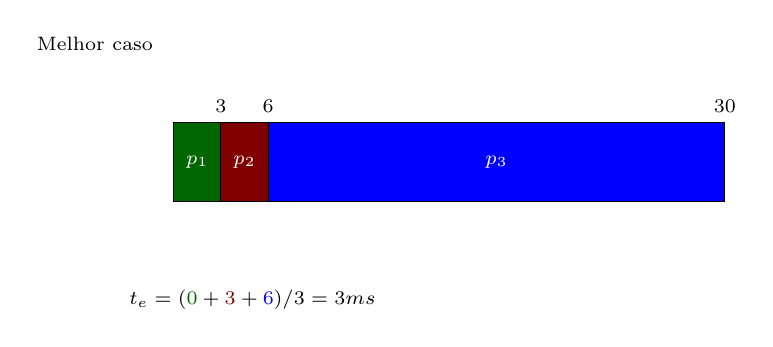
\begin{tikzpicture}[p1/.style={fill=\colorone},
  p23/.style={fill=\colortwo},
  labelsty/.style={midway,text=white}]
  \node at (-1,2) {\alert{Melhor} caso};
 
  \draw[p1] (0,0) rectangle (0.6,1) node[labelsty]{$p_1$} node[above]{3};
  \draw[p23] (0.6,0) rectangle (1.2,1) node[labelsty]{$p_2$}node[above]{6};
  \draw[p23,fill=\colorthree] (1.2,0) rectangle (7,1) node[labelsty]{$p_3$} node[above]{30};
  \node at (1,-1.25) {$t_e = ({\color{\colorone} 0 }+ {\color{\colortwo}3} + {\color{\colorthree}6} ) / 3 = 3 ms$};
\end{tikzpicture}
}
\end{frame}


\begin{frame}
\frametitle{Tarefa mais curta primeiro}
\framesubtitle{{\it SJF -- shortest job first}}

\def\max{3}
\def\pone{3/\max}
\def\ptwo{\pone + 6/\max}
\def\pthree{\ptwo + 7/\max}
\def\pfour{\pthree + 8/\max}

\begin{center}
\begin{tabular}{c|c} \hline
  processo & tempo de surto (ms) \\ \hline
  $p_1$ & 6 \\
  $p_2$ & 8 \\
  $p_3$ & 7 \\ 
  $p_4$ & 3 \\ \hline
\end{tabular}
\end{center}

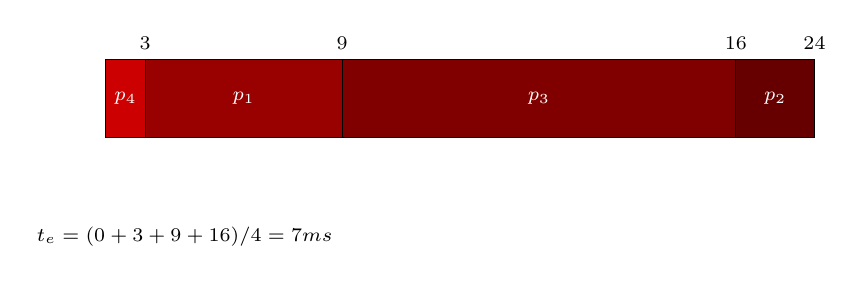
\begin{tikzpicture}[proc/.style={fill=red!80!black},
  labelsty/.style={midway,text=white}]
  \draw[proc,fill=red!80!black] (0,0) rectangle (\pone,1) node[labelsty]{$p_4$} node[above]{3};
  \draw[proc,fill=red!60!black] (\pone,0) rectangle (\ptwo,1) node[labelsty]{$p_1$} node[above]{9};
  \draw[proc,fill=red!50!black] (\ptwo,0) rectangle (\pthree,1) node[labelsty]{$p_3$} node[above]{16};
  \draw[proc,fill=red!40!black] (\pthree,0) rectangle (\pfour,1) node[labelsty]{$p_2$}node[above]{24};
  
  \node at (1,-1.25) {$t_e = (0 + 3  + 9 + 16) / 4 = 7 ms$};
  
\end{tikzpicture}

\end{frame}

\subsubsection{Sistemas interativos}
\label{subsection:interactive}

\begin{frame}
\frametitle{Escalonamento por prioridade}

\def\mmc{2}
\def\pone{1/\mmc}
\def\ptwo{\pone + 5/\mmc}
\def\pthree{\ptwo + 10/\mmc}
\def\pfour{\pthree + 2/\mmc}
\def\pfive{\pfour + 1/\mmc}

\begin{center}
\begin{tabular}{c|c|c} \hline
  processo & tempo de surto(ms) & prioridade \\ \hline
  $p_1$ & 10 & 3 \\
  $p_2$ & 1 & 1 \\
  $p_3$ & 2 & 4 \\ 
  $p_4$ & 1 & 5 \\ 
  $p_5$ & 5 & 2 \\ \hline
\end{tabular}
\end{center}

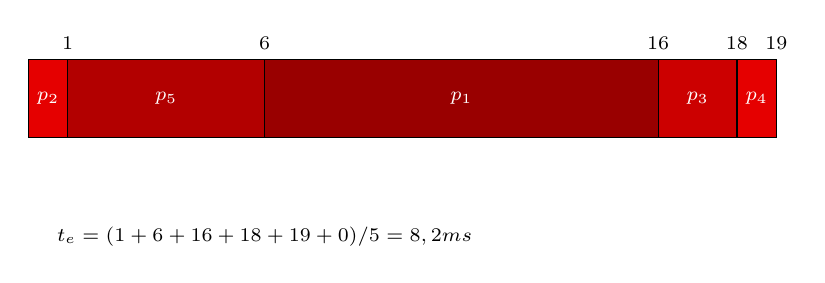
\begin{tikzpicture}[proc/.style={fill=red!90!black},
  labelsty/.style={midway,text=white}]
  \draw[proc] (0,0) rectangle (\pone,1) node[labelsty]{$p_2$} node[above]{1};
  \draw[fill=red!70!black] (\pone,0) rectangle (\ptwo,1) node[labelsty]{$p_5$} node[above]{6};
  \draw[fill=red!60!black] (\ptwo,0) rectangle (\pthree,1) node[labelsty]{$p_1$} node[above]{16};
  \draw[fill=red!80!black] (\pthree,0) rectangle (\pfour,1)  node[labelsty]{$p_3$}node[above]{18};
  \draw[proc] (\pfour,0) rectangle (\pfive,1) node[labelsty]{$p_4$}node[above]{19};
  
  \node at (3,-1.25) {$t_e = (1  + 6 + 16 + 18 + 19 + 0) / 5 = 8,2 ms$};
  
\end{tikzpicture}

\end{frame}


\begin{frame}{Escalonamento por {\em Round-Robin} (revezamento)}

\begin{center}
\begin{tabular}{c|c} \hline
  processo & tempo de surto (ms) \\ \hline
  {\color{\colorone} $p_1$} & 24 \\
  {\color{\colortwo}$p_2$} & 3 \\
  {\color{\colorthree}$p_3$} & 3  \\ \hline
\end{tabular}
\end{center}

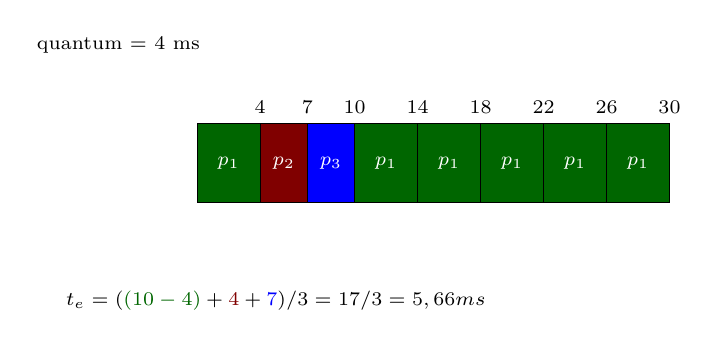
\begin{tikzpicture}[p1/.style={fill=\colorone},
  p23/.style={fill=\colortwo},
  labelsty/.style={midway,text=white}]
  \node at (-1,2) {\alert{quantum} $=$ $4$ ms};
  \draw[p1] (0,0) rectangle (.8,1) node[labelsty]{$p_1$} node[above]{4};
  \draw[p23] (.8,0) rectangle (1.4,1) node[labelsty]{$p_2$} node[above]{7};
  \draw[p23,fill=\colorthree] (1.4,0) rectangle (2.0,1)
  node[labelsty]{$p_3$}node[above]{10};
  \draw[p1] (2.0,0) rectangle (2.8,1) node[labelsty]{$p_1$} node[above]{14};
  \draw[p1] (2.8,0) rectangle (3.6,1) node[labelsty]{$p_1$}
  node[above]{18};
  \draw[p1] (3.6,0) rectangle (4.4,1) node[labelsty]{$p_1$}
  node[above]{22};
  \draw[p1] (4.4,0) rectangle (5.2,1) node[labelsty]{$p_1$}
  node[above]{26};
  \draw[p1] (5.2,0) rectangle (6,1) node[labelsty]{$p_1$} node[above]{30};
  \node at (1,-1.25) {$t_e = ({\color{\colorone} (10 - 4) }+
    {\color{\colortwo}4} + {\color{\colorthree}7} ) / 3 = 17/3 = 5,66 ms$};
\end{tikzpicture}

\end{frame}

\begin{frame}{Quantum x troca de contexto}

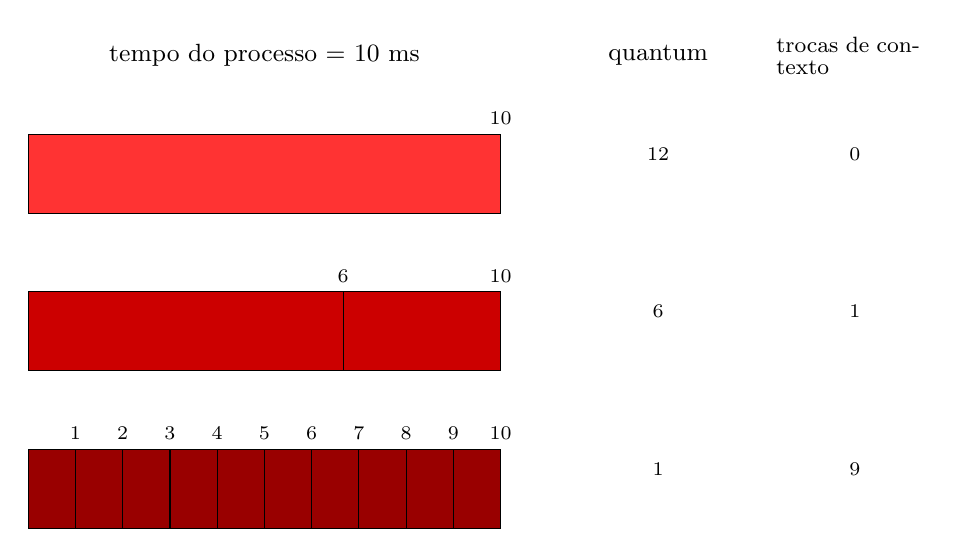
\begin{tikzpicture}[p1/.style={fill=\colorone},
  labelsty/.style={midway,text=white}]
  \node at (3,2) {\small tempo do processo $=$ $10$ ms};
  \node at (8,2) {\small quantum};
  \node[text width=2cm] at (10.5,2) {\footnotesize trocas de contexto};
 
  \draw[fill=red!80!white] (0,0) rectangle (6,1) node[labelsty]{} node[above]{10};
  \node at (8,0.75) {12};
  \node at (10.5,0.75) {0};

  \draw[fill=red!80!black] (0,-2) rectangle (4,-1)
  node[labelsty]{} node[above]{6};
  \draw[fill=red!80!black] (4,-2) rectangle (6,-1)
  node[labelsty]{} node[above]{10};
  \node at (8,-1.25) {6};
  \node at (10.5,-1.25) {1};

  \foreach \x/\i in {0/1,1/2,2/3,3/4,4/5,5/6,6/7,7/8,8/9,9/10} {
    \draw[fill=red!60!black] (\x/10*6,-4) rectangle (\x/10*6+0.6,-3) node[labelsty]{} node[above]{\i};
  }
  \node at (8,-3.25) {1};
  \node at (10.5,-3.25) {9};
\end{tikzpicture}

\end{frame}


\begin{frame}{Exercício 1}{Fonte: ``Sistemas Operacionais com Java'',
      Silberschatz, Galvin, Gagne. Ed. Campus, 2008.}
  \footnotesize
  Considere os seguintes processos com o tempo de execução ({\em burst}) no
  processador data em milisegundos:
  \begin{center}
  \begin{tabular}{ccc}\hline
    Processo & tempo de execução & prioridade \\\hline
    p$_1$ & 10 & 3\\
    p$_2$ & 1 & 1 \\
    p$_3$ & 2 & 3 \\
    p$_4$ & 1 & 4 \\
    p$_5$ & 5 & 2 \\\hline
  \end{tabular}
\end{center}
Considere que os processos chegaram na ordem p$_1$, p$_2$, p$_3$,
p$_4$, p$_5$, todos no momento $0$.
\begin{itemize}
\item Desenhe quatro gráficos de Gantt para a utilização das seguintes
  políticas de escalonamento: FIFO, SJF, prioridade preemptivo e
  revezamento (Round-Robin) com quantum igual a $1$ ms.
\item Qual o tempo de espera para cada processo para cada uma das políticas?
\item Qual o tempo de espera médio?
\end{itemize}

\end{frame}



\begin{frame}{Escalonamento com fila de multinível}
\framesubtitle{Escalonamento {\em multilevel queue}}

 \begin{tikzpicture}
   \tikzset{inout/.style={single arrow, minimum height=2cm,
       anchor=west,fill=green!50!black,draw}}

   \node at (0,1) {Nível mais alto};
   \node at (0,-5.5) {\footnotesize Nível mais baixo};

   \foreach \dy/\nome in {0/sistema,1.5/interativo,3/{edição
       interativa},4.5/{lote ({\em batch})}} {
     \node[inout] at (0,0-\dy) {};
     \draw[fill=red!80!black] (2,-0.5-\dy) rectangle (6,0.5-\dy)
     node[anchor=north east]{\nome};
     \node[inout] at (6,0-\dy) {};
   }
\end{tikzpicture}
  
\end{frame}

\begin{frame}{Escalonamento {\em multilevel feedback-queue}}
  
  \begin{tikzpicture}[shorten >=1pt,node distance=2cm,on grid]
    \tikzset{level/.style={anchor=west,shape=cylinder,minimum width=0.75cm,minimum
        height=3cm,draw},thelabel/.style={font=\small},
    thearrow/.style={->,>=latex,draw}}
    \node[level] at (2,0) {quantum=8}; 
    \node[level] at (2,-2) {quantum=16}; 
    \node[level] at (2,-4)  {FCFS};

    \draw[thearrow] node[thelabel,anchor=south] {entrada} (0,0) --
    (2,0) node[anchor=south east] {\footnotesize fila 0};
    \draw[thearrow] (4.75,0.25) -- +(2,0);
    \draw[thearrow] (4.75,-0.25) -- +(2,0) -- +(2,-1) -- +(-4,-1) --
    +(-4,-1.75) -- +(-2.75,-1.75) node[anchor=south east] {\footnotesize fila 1};
    
    \draw[thearrow] (4.75,-1.75) -- +(2,0);
    \draw[thearrow] (4.75,-2.25) -- +(2,0) -- +(2,-1) -- +(-4,-1) --
    +(-4,-1.75) -- +(-2.75,-1.75) node[anchor=south east] {\footnotesize fila 2};
    
    \draw[thearrow] (4.75,-4) -- +(2,0);

  \end{tikzpicture}
\bigskip
\small
  \begin{enumerate}
  \item Fila 0 $\rightarrow$ quantum$_{\text{processo}}$ $\leq$ $8$;
  \item Fila 1 $\rightarrow$ quantum$_{\text{processo}}$ $\leq$ $24$;
  \item Fila 2 $\rightarrow$ quantum$_{\text{processo}}$ $>$ $24$.
  \end{enumerate}

\end{frame}


%%% MULTIPLOS PROCESSADORES
\def\thetitle{Escalonamento em múltiplos processadores}
\title{\thetitle}
\frame{\date{}\author{}\titlepage}
\subsection{\thetitle}

\begin{frame}{Técnicas de escalonamento com multiprocessadores}

  \begin{itemize}
  \item \alert{Multiprocessamento assimétrico} -- todas as atividades de
    escalonamento, processamento de E/S são tratadas por um
    processador único, o servidor mestre. Simples pelo fato de
    possibilitar acesso único aos dados compartilhados.
    \pause
  \item \alert{Multiprocessamento simétrico} (SMP\footnote{{\em
        Symmetric Multiprocessing}}) -- cada processador é
    auto-escalonado, podendo ter sua própria fila de processos prontos
    ou compartilhar uma fila comum. O escalonador, porém, é específico
    para cada processador devendo examinar as filas de pronto e tomar
    cuidado com as estruturas de dados compartilhadas com outros
    processadores. Ex: Windows XP, Linux, Solaris, Mac OS X.
  \end{itemize}
  
\end{frame}


\begin{frame}{Afinidade do processador}{SMP}
  
  Atribui um processo específico a um processador reduzindo o custo de
  transferência dos dados da memória \alert{cache} de um processador
  para outro, além da invalidação dos dados na memória \alert{cache}
  do primeiro processador.

  \begin{itemize}
  \item \alert{Afinidade flexível} -- processo pode migrar;
  \item \alert{Afinidade rígida} -- processo não pode migrar (Ex: Linux).
  \end{itemize}

\end{frame}

\begin{frame}{Multithreading simétrico}{SMT}

A tecnologia de {\em Multithreading simétrico}(SMT\footnote{\em
Symmetric Multithreading}) fornece vários processadores lógicos em um
único processador físico.

Cada processador possui seu próprio \alert{estado arquitetônico} que inclui
registradores de uso geral e de estado de máquina.
  
Como SMT é um recurso implementado em hardware, o sistema operacional
não precisa \alert{necessariamente} gerenciar o escalonamento dos processos.

\end{frame}

%%% EXEMPLOS
\def\thetitle{Exemplos}
\title{\thetitle}
\frame{\date{}\author{}\titlepage}

\subsection{\thetitle}

\begin{frame}{Escalonamento no Windows XP}

  \begin{itemize}
  \item Escalonamento com base em \alert{prioridade} e
    \alert{preemptivo};
    \begin{itemize}
    \item \alert{\em Thread} de maior prioridade sempre será executada.
    \end{itemize}
    \pause
  \item O \alert{despachante} pode interromper a {\em thread} em
    execução de acordo com as seguintes condições:
    \begin{itemize}
    \item Término de execução da {\em thread};
    \item Término de quantum de tempo da {\em thread};
    \item Requisição de execução de uma {\em thread} de maior prioridade;
    \item Invocação de uma chamada de sistema bloqueante (E/S, por exemplo).
    \end{itemize}
    \pause
  \item Esquema de prioridade: $0 \rightarrow 31$.
    \begin{enumerate}
    \item Classe variável: $1 \rightarrow 15$.
    \item Classe de tempo real: $16 \rightarrow 31$.
    \item Prioridade $0$: usada pelo sistema para gerenciamento de memória.
    \end{enumerate}
  \end{itemize}
  
\end{frame}



\begin{frame}[fragile]{Escalonamento no Windows XP}{Classes de prioridades}
\footnotesize
  
\begin{tikzpicture}
  \tikzset{every node/.style={font=\scriptsize},thrdcls/.style={cylinder,anchor=east,draw},changes/.style={<->,>=latex}}
    
  % classes
  \node[draw] at (-5.35,5.75) {\color{gray}Classes de proridade};
    \node[thrdcls,fill=black!80!red,font={\color{white}}] (rt) at (-3,5)
    {REALTIME\_PRIORITY\_CLASS};
    \node[thrdcls,fill=black!40!red] (high) at (-3,4)
    {HIGH\_PRIORITY\_CLASS};
    \node[thrdcls,fill=black!30!red] (above) at (-3,3)
    {ABOVE\_NORMAL\_PRIORITY};
    \node[thrdcls,fill=black!20!red] (normal) at (-3,2) {NORMAL\_PRIORITY\_CLASS};
    \node[thrdcls,fill=black!10!red] (below) at (-3,1)
    {BELOW\_NORMAL\_PRIORITY\_CLASS};
        \node[thrdcls] (idle) at (-3,0) {IDLE\_PRIORITY\_CLASS};

        % caminhos
        \draw [changes] (high.west) .. controls +(left:15mm) and +(left:5mm)
        .. (above.west);
        \draw [changes] (above.west) .. controls +(left:5mm) and +(left:5mm)
        .. (normal.west);
        \draw [changes] (normal.west) .. controls +(left:15mm) and +(left:5mm)
        .. (below.west);
        \draw [changes] (below.west) .. controls +(left:5mm) and +(left:15mm)
        .. (idle.west);
        
        % despachante
        \draw[<-,>=latex] (-9.5,-1) -- (-9.5,6) node[above right,draw] {\color{gray}despachante};

        % tabela de valores relativos
        \node[draw] at (0,6.5) {\color{gray}Valores relativos};
        \def\xa{-2}\def\xb{-0.5}\def\xc{1} \def\xd{1.9} \foreach \x/\v
        in {\xa/\only<1>{\tiny TIME\_CRITICAL},\xb/\only<1>{\tiny
            HIGHEST},\xc/\only<1>{\tiny
            ABOVE\_NORMAL},\xa/\only<2>{\tiny
            NORMAL},\xb/\only<2>{{\tiny BELOW\_NORMAL}},
          \xc/\only<2>{\tiny LOWEST}, \xd/\only<2>{\tiny IDLE}}{\node
          at (\x,6) {\v};} \foreach \x/\v in
        {\xa/\only<1>{31},\xb/\only<1>{26},\xc/\only<1>{25},\xa/\only<2>{\color{blue}24},\xb/\only<2>{23},\xc/\only<2>{22},\xd/\only<2>{16}}{\node
          at (\x,5){\v};} \foreach \x/\v in
        {\xa/\only<1>{15},\xb/\only<1>{15},\xc/\only<1>{14},\xa/\only<2>{\color{blue}13},\xb/\only<2>{12},\xc/\only<2>{11},\xd/\only<2>{1}}{\node
          at (\x,4) {\v};} \foreach \x/\v in
        {\xa/\only<1>{15},\xb/\only<1>{12},\xc/\only<1>{11},\xa/\only<2>{\color{blue}10},\xb/\only<2>{9},\xc/\only<2>{8},\xd/\only<2>{1}}{\node
          at (\x,3) {\v};} \foreach \x/\v in
        {\xa/\only<1>{15},\xb/\only<1>{10},\xc/\only<1>{9},\xa/\only<2>{\color{blue}8},\xb/\only<2>{7},\xc/\only<2>{6},\xd/\only<2>{1}}{\node
          at (\x,2) {\v};} \foreach \x/\v in
        {\xa/\only<1>{15},\xb/\only<1>{8},\xc/\only<1>{7},\xa/\only<2>{\color{blue}6},\xb/\only<2>{5},\xc/\only<2>{4},\xd/\only<2>{1}}{\node
          at (\x,1) {\v};} \foreach \x/\v in
        {\xa/\only<1>{15},\xb/\only<1>{6},\xc/\only<1>{5},\xa/\only<2>{\color{blue}4},\xb/\only<2>{3},\xc/\only<2>{2},\xd/\only<2>{1}}{\node
          at (\x,0) {\v};}

        % prioridade basica
        
        \draw<2>[<-,>=latex,color=blue] (-2,-.2) -- (-2,-1) node[above
        right,draw] {\color{blue}\scriptsize prioridade básica};

  \end{tikzpicture}
\end{frame}

\begin{frame}{Regras de escalonamento}{Windows XP}

  \begin{itemize}
  \item<1-| alert@1> Processos são membros de {\tt NORMAL\_PRIORITY\_CLASS},
    exceto:
    \begin{itemize}
    \item Quando o processo pai pertence a {\tt IDLE\_PRIORITY\_CLASS}
      {\em ou};
    \item Quando foi especificada outra classe na criação do processo.
    \end{itemize}
  \item<2-| alert@2> Quando o quantum de tempo de uma {\em thread} se esgota, esta
    é interrompida e se a classe de prioridade for variável, sua
    prioridade é reduzida, porém, nunca menos do que a prioridade básica.
  \item<3-| alert@3> Quando um processo pertence à classe {\tt
      NORMAL\_PRIORITY\_CLASS}, e está atualmente selecionado na tela
    (primeiro plano), seu quantum é aumentado, obtendo mais tempo de
    execução antes de ser preemptado.
  \item<4-| alert@4> A classe {\tt REALTIME\_PRIORITY\_CLASS} é invariante e
    provoca preempção de outros processos quando volta para a fila pronto.

  \end{itemize}
  
\end{frame}

\subsection{Exercício}

\begin{frame}{Exercício 2}{Fonte: ``Sistemas Operacionais''. Oliveira,
    Carissimi, Toscani. Ed. Bookman, 2008.}

\small
Quatro programas devem ser executados em um computador. Todos os
programas são compostos por 2 ciclos de processador e 2 ciclos de
E/S. A entrada e saída de todos os programas é feita sobre a mesma
unidade de disco. Os tempos para cada ciclo de cada programa são
mostrados abaixo:

\begin{center}
  \begin{tabular}{ccccc}\hline
    programa & processador & disco & processador & disco \\\hline
    p$_1$ & 3 & 10 & 3 & 12 \\
    p$_2$ & 4 & 12 & 6 & 8 \\
    p$_3$ & 7 & 8 & 8 & 10 \\
    p$_4$ & 6 & 14 & 2 & 10 \\\hline
  \end{tabular}
\end{center}
Construa um diagrama de tempo mostrando qual programa está ocupando o
processador e o disco a cada momento, até que os 4 programas
terminem. Suponha que a política utilizada seja o de revezamento
(Round-Robin), com quantum de 4 unidades. Qual a taxa de ocupação do
processador e do disco?

\end{frame}
